
\chapter{Experiments} % Main chapter title

\label{ch:05} % Change X to a consecutive number; for referencing this chapter elsewhere, use \ref{ChapterX}


The model is trained with PyTorch 1.10.2, CUDA 10.2.89, GPU with single NVIDIA GEFORCE GTX 1080Ti.


%% nnnn exp
\section{Gated Convolution Neural Network for Normal Inference}

The first neural network that worked well for normal prediction in this master thesis is introduced in this section. It is named Gated Convolution Neural Network, or GCNN. The GCNN model is nothing but a UNet with gated convolution layers. it can predict normal map based on a point cloud. The error is around 10 degrees.

The model uses a 512x512x3 3D vertex matrix as input and the output is a 512x512x3 normal map. The architecture is based on description in \ref{sec:architecture}. The channel size is up to 32 through the whole network. For the training parameters, learning rate is 0.001, penalty is 1.4, optimizer is Adam optimizer, the loss function is penalty-l2 loss as described in \ref{sec:loss}.




The evaluation result on 90 test scenes is shown in Figure \ref{fig:scatter-gcnn}.
The GCNN based method has angle error between 5 to 15 degrees in both type of inputs. The error trends to higher with point number decrease. It is because the less points in the point cloud, the more detail is hided due to the insufficient of resolution. Therefore the recorded surface based on the point cloud is more coarse, which also increase the difficulty of the normal inference.

\begin{figure}[h!]
	\centering
	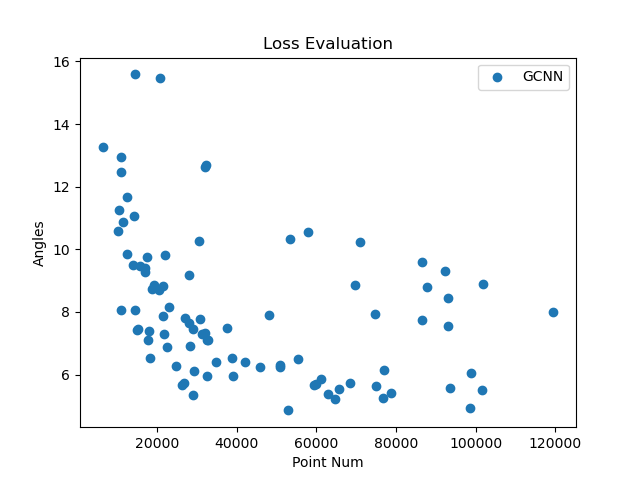
\includegraphics[width=.4\textwidth]{./Figures/scatter-gcnn-no-noise.png}
	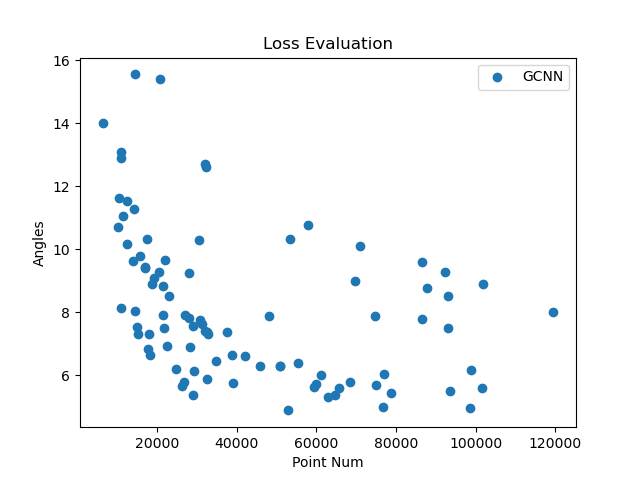
\includegraphics[width=.4\textwidth]{./Figures/scatter-gcnn-noised.png}
	\caption{Evaluation of average angular loss on the whole test dataset with 90 scenes. The x-axis indicates the point number, the y-axis indicates the angles. The \textbf{Left} one using point cloud without noise, the \textbf{right} one has noise.}
	\label{fig:scatter-gcnn}
\end{figure}

The evaluation visualization on synthetic dataset is shown in Figure \ref{fig:gcnn-eval-synthetic}. The error concentrate mainly on severe changed surface region, like the teeth, paw and horn of the dragon.
\begin{figure}[h!]
	\centering
	\begin{subfigure}[b]{0.24\linewidth}
		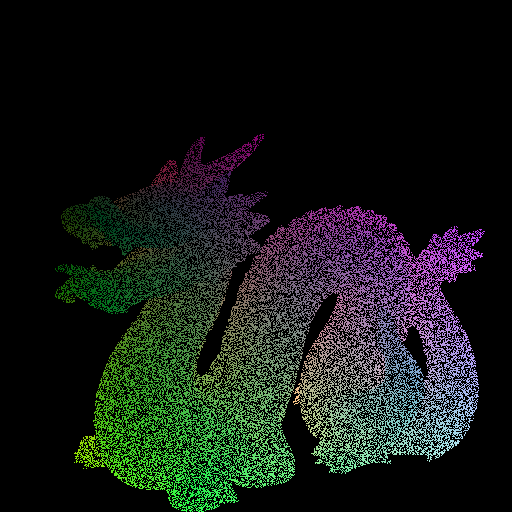
\includegraphics[width=\linewidth]{./Figures/gcnn-synthetic/fancy_eval_3_point_cloud_noise.png}
		\caption{point cloud}
	\end{subfigure}
	\begin{subfigure}[b]{0.24\linewidth}
		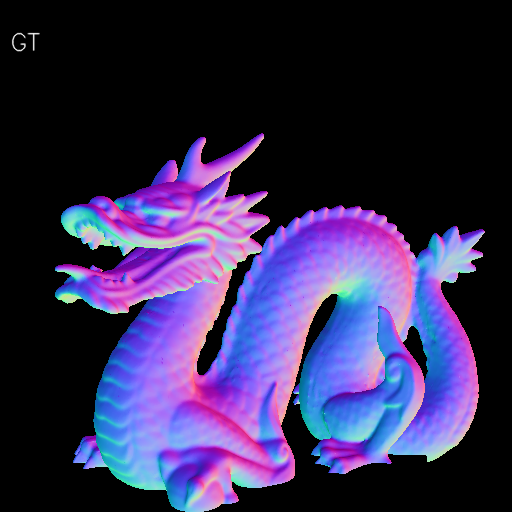
\includegraphics[width=\linewidth]{./Figures/gcnn-synthetic/fancy_eval_3_groundtruth.png}
		\caption{ground-truth}
	\end{subfigure}
	\begin{subfigure}[b]{0.24\linewidth}
		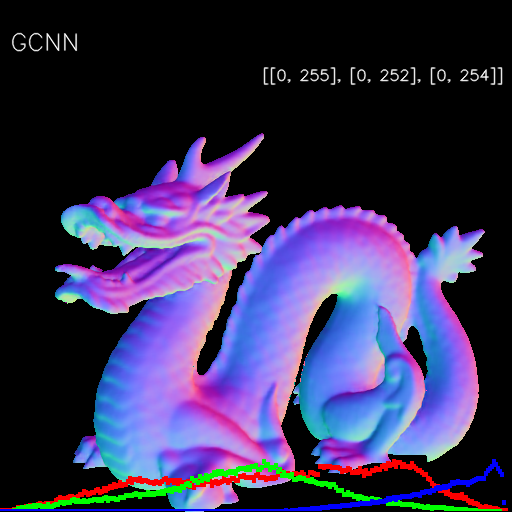
\includegraphics[width=\linewidth]{./Figures/gcnn-synthetic/fancy_eval_3_normal_GCNN.png}
		\caption{GCNN}
	\end{subfigure}
	\begin{subfigure}[b]{0.24\linewidth}
		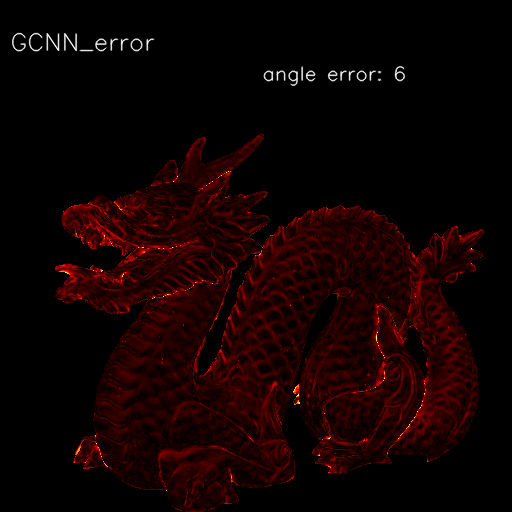
\includegraphics[width=\linewidth]{./Figures/gcnn-synthetic/fancy_eval_3_error_GCNN.png}
		\caption{Angle Error}
	\end{subfigure}
	\caption{GCNN Normal Inference on Synthetic Dataset (object: dragon)}
	\label{fig:gcnn-eval-synthetic}
\end{figure}


The evaluation visualization on real dataset is shown in Figure \ref{fig:gcnn-eval-real}
\begin{figure}[h!]
	\centering
	\begin{subfigure}[b]{0.24\linewidth}
		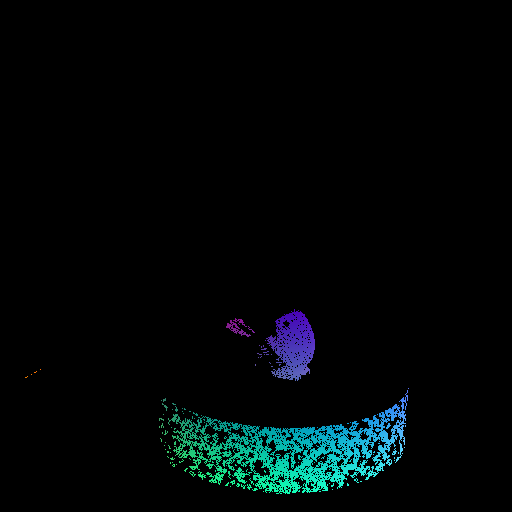
\includegraphics[width=\linewidth]{./Figures/gcnn-real/fancy_eval_1_point_cloud_noise.png}
		\caption{point cloud}
	\end{subfigure}
	\begin{subfigure}[b]{0.24\linewidth}
		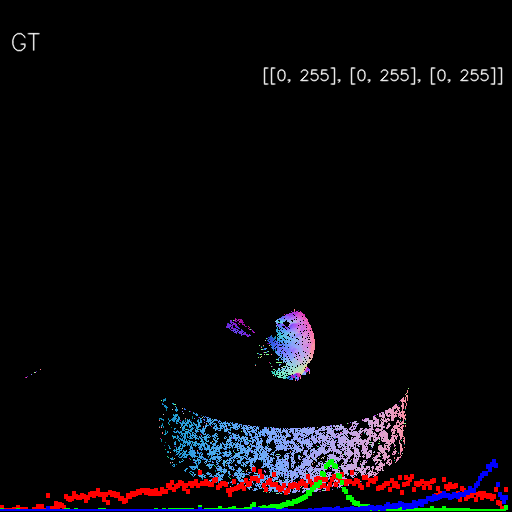
\includegraphics[width=\linewidth]{./Figures/gcnn-real/fancy_eval_1_groundtruth.png}
		\caption{ground-truth}
	\end{subfigure}
	\begin{subfigure}[b]{0.24\linewidth}
		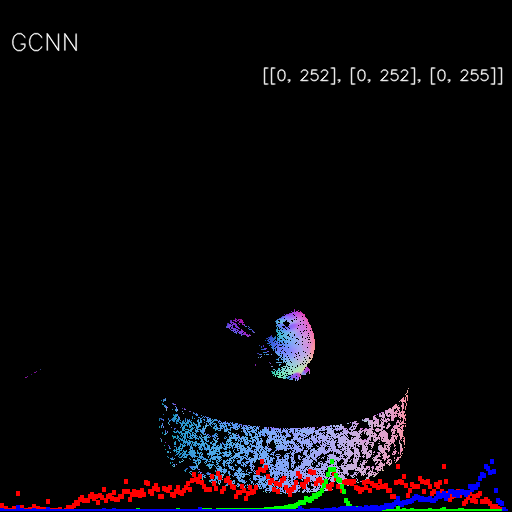
\includegraphics[width=\linewidth]{./Figures/gcnn-real/fancy_eval_1_normal_GCNN.png}
		\caption{GCNN}
	\end{subfigure}
	\begin{subfigure}[b]{0.24\linewidth}
		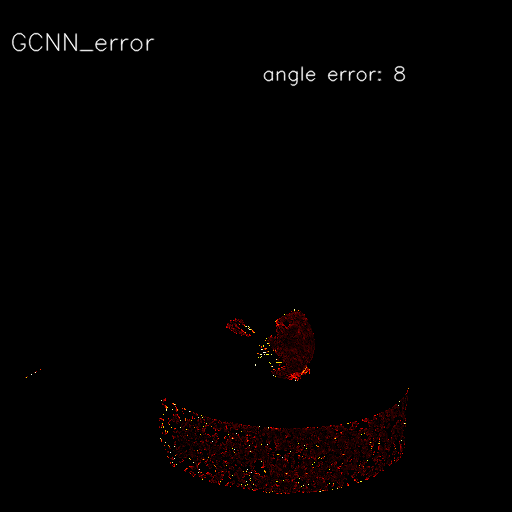
\includegraphics[width=\linewidth]{./Figures/gcnn-real/fancy_eval_1_error_GCNN.png}
		\caption{Angle Error}
	\end{subfigure}
	\caption{Evaluation on Real Dataset}
	\label{fig:gcnn-eval-real}
\end{figure}



%% resng
\section{Guided Gated Convolution Neural Network for Normal Inference }

The inference result of guided-GCNN model is shown in Figure \ref{fig:ng-eval-synthetic}. With adding the information of a gray-scale image, the model is able to sharpen the details over the whole scene. 

\begin{figure}[h!]
	\centering
	\begin{subfigure}[b]{0.19\linewidth}
		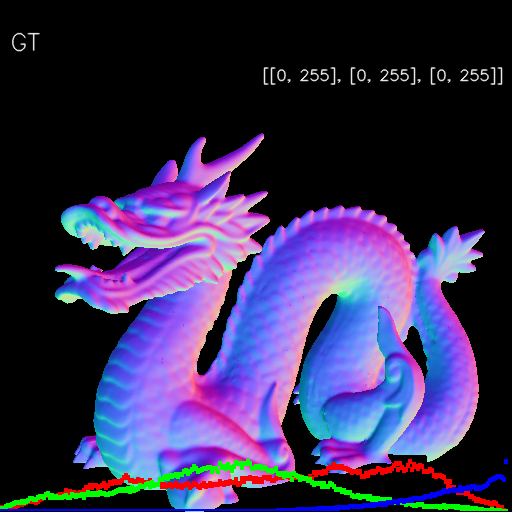
\includegraphics[width=\linewidth]{./Figures/ng-synthetic/fancy_eval_3_groundtruth.png}
		\caption{GT}
	\end{subfigure}
	\begin{subfigure}[b]{0.19\linewidth}
		\includegraphics[width=\linewidth]{./Figures/ng-synthetic/fancy_eval_3_normal_NG.png}
		\caption{g-GCNN}
	\end{subfigure}
	\begin{subfigure}[b]{0.19\linewidth}
		\includegraphics[width=\linewidth]{./Figures/ng-synthetic/fancy_eval_3_error_NG.png}
		\caption{Angle Error}
	\end{subfigure}
	\begin{subfigure}[b]{0.19\linewidth}
		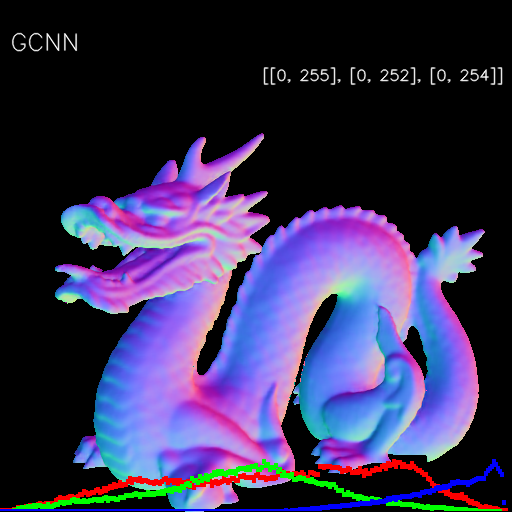
\includegraphics[width=\linewidth]{./Figures/gcnn-synthetic/fancy_eval_3_normal_GCNN.png}
		\caption{GCNN}
	\end{subfigure}
	\begin{subfigure}[b]{0.19\linewidth}
		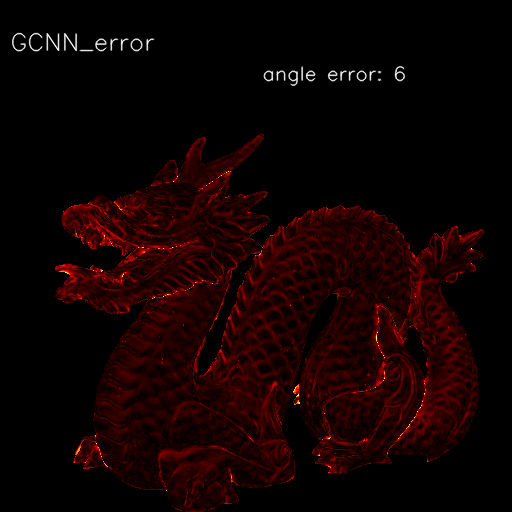
\includegraphics[width=\linewidth]{./Figures/gcnn-synthetic/fancy_eval_3_error_GCNN.png}
		\caption{Angle Error}
	\end{subfigure}
	\caption{guided-GCNN Normal Inference on Synthetic Dataset (object: dragon). GCNN result is shown on (d) and (e) as comparison.}
	\label{fig:ng-eval-synthetic}
\end{figure}


\newpage 
\section{model comparison}
This section evaluates the proposed models with the neighbor-based model and make comparison with each other.

\begin{figure}[h!]
	\centering
	\begin{subfigure}[b]{0.24\linewidth}
		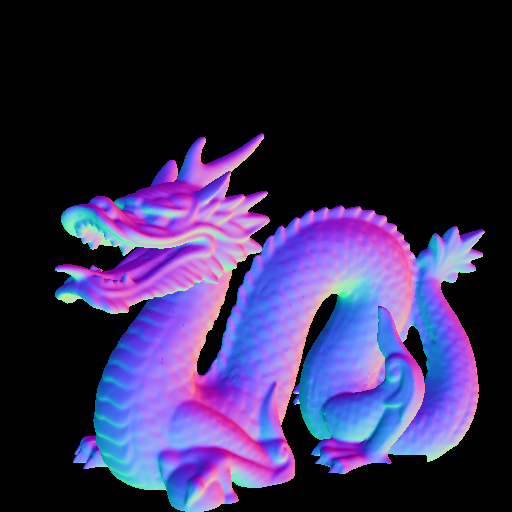
\includegraphics[width=\linewidth]{./Figures/comparison/fancy_eval_3_groundtruth.png}
		\caption{ground-truth}
	\end{subfigure}
	\begin{subfigure}[b]{0.24\linewidth}
		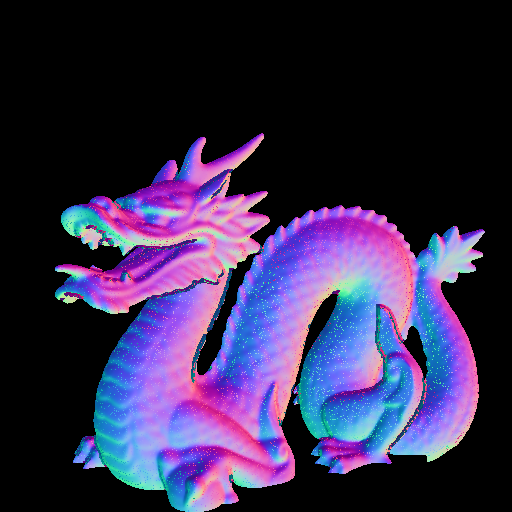
\includegraphics[width=\linewidth]{./Figures/comparison/fancy_eval_3_normal_svd.png}
		\caption{SVD}
	\end{subfigure}
	\begin{subfigure}[b]{0.24\linewidth}
		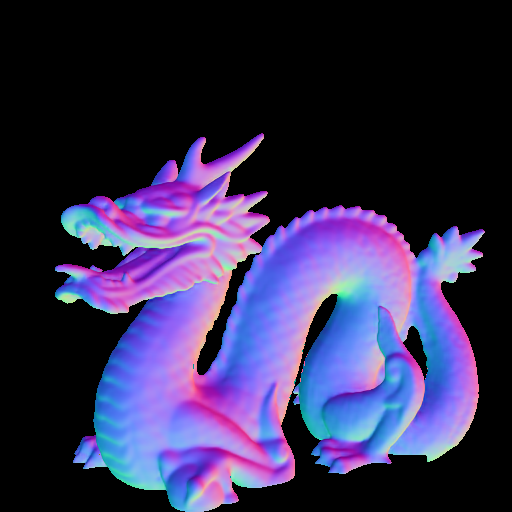
\includegraphics[width=\linewidth]{./Figures/comparison/fancy_eval_3_normal_GCNN.png}
		\caption{GCNN}
	\end{subfigure}
	\begin{subfigure}[b]{0.24\linewidth}
		\includegraphics[width=\linewidth]{./Figures/comparison/fancy_eval_3_normal_NG.png}
		\caption{guided-GCNN}
	\end{subfigure}
	
	\begin{subfigure}[b]{0.3\linewidth}
		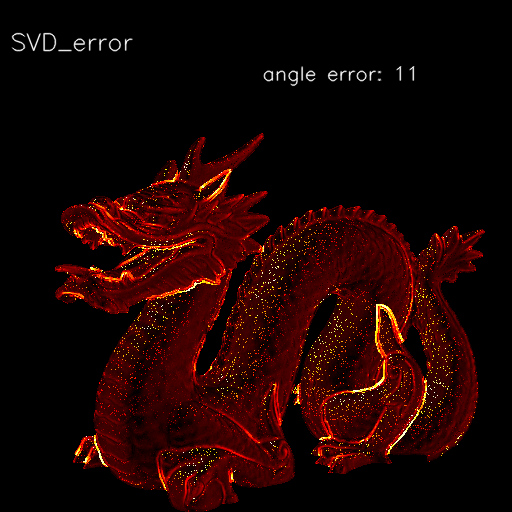
\includegraphics[width=\linewidth]{./Figures/comparison/fancy_eval_3_error_SVD.png}
		\caption{Error}
	\end{subfigure}
	\begin{subfigure}[b]{0.3\linewidth}
		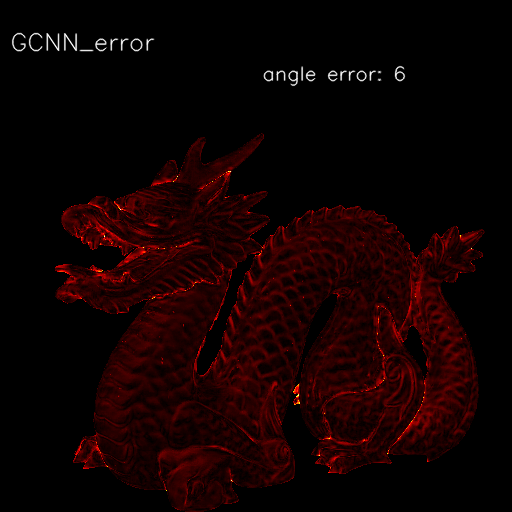
\includegraphics[width=\linewidth]{./Figures/comparison/fancy_eval_3_error_GCNN.png}
		\caption{Error}
	\end{subfigure}
	\begin{subfigure}[b]{0.3\linewidth}
		\includegraphics[width=\linewidth]{./Figures/comparison/fancy_eval_3_error_NG.png}
		\caption{Error}
	\end{subfigure}
	
	\caption{Normal Inference on different models with errors. (object: dragon)}
	\label{fig:eval-svd}
\end{figure}
